% diagrams/english/cocina.tex -- la cocina de los Brown, para "Where is
% it?": la ventana, la mesa con un bol grande encima, y el horno con una
% balda en la pared, por encima.
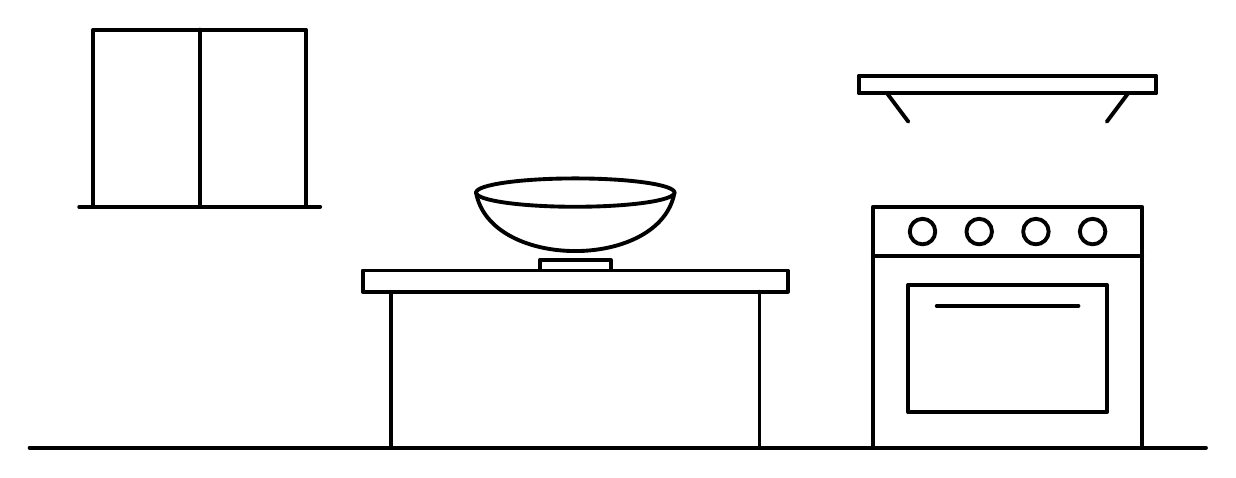
\begin{tikzpicture}[line width=1.4pt, line cap=round, line join=round, scale=0.9]
  \draw (-0.3,0) -- (16.3,0);
  % la ventana
  \filldraw[fill=white] (0.6,3.4) rectangle (3.6,5.9);
  \draw (2.1,3.4) -- (2.1,5.9); \draw (0.4,3.4) -- (3.8,3.4);
  % la mesa y el bol
  \filldraw[fill=white] (4.4,2.2) rectangle (10.4,2.5);
  \draw (4.8,2.2) -- (4.8,0); \draw (10.0,2.2) -- (10.0,0);
  \filldraw[fill=white] (6.9,2.5) rectangle (7.9,2.65);
  \filldraw[fill=white] (6.0,3.6) .. controls (6.2,2.5) and (8.6,2.5) .. (8.8,3.6) -- cycle;
  \filldraw[fill=white] (7.4,3.6) ellipse (1.4 and 0.2);
  % el horno
  \filldraw[fill=white] (11.6,0) rectangle (15.4,3.4);
  \draw (11.6,2.7) -- (15.4,2.7);
  \foreach \x in {12.3,13.1,13.9,14.7} { \filldraw[fill=white] (\x,3.05) circle (0.18); }
  \filldraw[fill=white] (12.1,0.5) rectangle (14.9,2.3);
  \draw (12.5,2.0) -- (14.5,2.0);
  % la balda, encima del horno
  \filldraw[fill=white] (11.4,5.0) rectangle (15.6,5.25);
  \draw (11.8,5.0) -- (12.1,4.6); \draw (15.2,5.0) -- (14.9,4.6);
\end{tikzpicture}
